% TEMPLATE for Usenix papers, specifically to meet requirements of
%  USENIX '05
% originally a template for producing IEEE-format articles using LaTeX.
%   written by Matthew Ward, CS Department, Worcester Polytechnic Institute.
% adapted by David Beazley for his excellent SWIG paper in Proceedings,
%   Tcl 96
% turned into a smartass generic template by De Clarke, with thanks to
%   both the above pioneers
% use at your own risk.  Complaints to /dev/null.
% make it two column with no page numbering, default is 10 point

% Munged by Fred Douglis <douglis@research.att.com> 10/97 to separate
% the .sty file from the LaTeX source template, so that people can
% more easily include the .sty file into an existing document.  Also
% changed to more closely follow the style guidelines as represented
% by the Word sample file. 

% Note that since 2010, USENIX does not require endnotes. If you want
% foot of page notes, don't include the endnotes package in the 
% usepackage command, below.

\documentclass[letterpaper,twocolumn,10pt]{article}
\usepackage{custom}
\usepackage{usenix,epsfig,endnotes,hyperref}
\usepackage{color, enumitem}
\usepackage{cleveref, float, graphicx, longtable, subcaption}

\begin{document}

%don't want date printed
\date{}

%make title bold and 14 pt font (Latex default is non-bold, 16 pt)
\title{\Large \bf Detection and Analysis of Disaster-Related Tweets}

\author{
{\rm Daniel Solomon}\\
\normalsize{\texttt{solomond@mail.tau.ac.il}}
\and
{\rm Gal Ron}\\
\normalsize{\texttt{galr1@mail.tau.ac.il‬}}
\and
{\rm Omri Ben-Horin}\\
\normalsize{\texttt{omribenhorin@mail.tau.ac.il}}
}

\maketitle

% Use the following at camera-ready time to suppress page numbers.
% Comment it out when you first submit the paper for review.
\thispagestyle{empty}


\abstract{}

\paragraph{}
\begin{center}
	\parbox{200pt}{
		Twitter has become an important channel of communication during times of emergency and disasters; it allows individuals to publish user-created content written in colloquial language, and update others on events from around the world.
		In this paper we present our work on disaster-related tweets using tools from the NLP pipeline, such as part-of-speech (POS) tagging and named-entity recognition (NER). We used a publicly available labeled dataset of tweets, and integrated our own classification tools together with Twitter-specific publicly available NLP tools, to create a classifier that reaches ~94\% accuracy in identifying disaster-related tweets. We also present an additional classifier trained to distinguish between "objective" disaster-related tweets and "subjective" ones. Lastly, we used NER to extract information on disasters, and experimented with  tweets recently sent from locations where natural disasters have occurred.
	
		Our code is available at: \url{https://github.com/glrn/nlp-disaster-analysis}.
	}
\end{center}

%%%%%%%%%%%%%%%%%%%%%%%%%%%%%%%%%%%%%%%%%%
\section{Introduction}
The popular microblogging service Twitter is a fruitful source of user-created content. With hundreds of millions of new tweets every day, Twitter has become a probe to human behavior and opinions from around the globe. The Twitter 'corpus' reflects political and social trends, popular culture, global and local happenings, and more. In addition, tweets are easy to access and aggregate in real-time. Therefore, we experience an increased interest in natural language processing research of Twitter data.

As one of the world's most widely used social networks, Twitter is an effective channel of communication and plays an important role during a crisis or emergency. The live stream of tweets can be used to identify reports and calls for help in emergency situations, such as accidents, violent crimes, natural disasters and terror attacks (which we all refer to as 'disasters' in this paper).

In this work we utilize techniques from the natural language processing pipeline (tokenization, part-of-speech tagging and named-entity recognition) to work on Twitter data, as opposed to traditional corpora, in order to detect and analyze disaster-related tweets.

\paragraph{The Dataset}
We present our experiments on a \href{https://www.crowdflower.com/data-for-everyone/}{dataset} of 10,877 tweets\endnote{\textbf{"Disasters on social media" Dataset by CrowdFlower}: Contributors looked at over 10,000 tweets culled with a variety of searches like "ablaze", "quarantine", and "pandemonium", then noted whether the tweet referred to a disaster. \url{https://www.crowdflower.com/wp-content/uploads/2016/03/socialmedia-disaster-tweets-DFE.csv}}, labeled to \textit{'disaster-related'} and \textit{'not disaster-related'} with confidence in the range $[0,1]$. For example, the following tweet is \textit{'disaster-related'} with confidence 1,

\begin{center}
	\parbox{190pt}{\tweet{Thunderstorms with little rain expected in Central California. High fire danger. \#weather \#cawx http://t.co/A5GNzbuSqq}}
\end{center}


while the following tweet is \textit{'not disaster-related'} with confidence 0.59,

\begin{center}
	\parbox{190pt}{\tweet{It's been raining since you left me // Now I'm drowning in the flood // You see I've always been a fighter // But without you I give up}}
\end{center}

Even for one who is not familiar with the Bon Jovi lyrics in the latter tweet, it is clear that the tweet does not refer to a real natural disaster. However, this observation is hard to make examining only the vocabulary used; the tweet contains a variety of 'disastrous' words  (\tweet{raining, drowning, flood, fighter}). This example hints that in order to reach meaningful results we may have to examine additional linguistic features of colloquial writing,  as well as Twitter-specific features such as hashtags (\tweet{\textbf{\#}}), user at-mentions (\tweet{\textbf{@}}), internet links and emoticons.


\paragraph{Our Contribution}

In this paper we present our work tackling three missions involving disaster-related tweets.

The first mission is \textit{identification} of disaster-related tweets among a variety of tweets. We implemented several classifiers, the best of which achieved around 94\% accuracy on the dataset. We note that this method could have easily been adjusted to identify tweets related to themes other than disasters (e.g. politics-related, sports-related, etc.), given the appropriate dataset. This part of our work is described in section \ref{mission1}.

The second mission is binary classification of disaster-related tweets to one of two categories, \textit{subjective tweets} (i.e. tweets that express an emotion) vs. \textit{objective tweets} (such as news reports on disasters). To achieve this we manually tagged 2,100 disaster-related tweets. The motivation behind this task is that objective tweets, such as informative news reports, are likely to be published after the event had already become clear to emergency services, while subjective tweets may contain invaluable first-person testimonies of ongoing events. This part of our work is described in section \ref{mission2}

Finally, we extracted named entities to enrich our knowledge on the disaster, comparing two NER methods (Twitter-oriented vs. general one). This part of our work is described in section \ref{mission3}.

To demonstrate our framework we aggregated recent tweets from various locations in the US, extracted disaster-related tweets using our classifier, and then used named-entity recognition to discover entities related to ongoing disasters. For example, "\tweet{Hurricane Harvey}" appeared as a top named-entity among recent tweets sent from Houston, TX, which we identified as \textit{disaster-related}. Further examples of results on recent data are presented in section \ref{recent-tweets-results}.

\subsection{Twitter vs. Traditional Corpora}

Tweets are limited to 140 characters and are widely used by non-professional writers. Therefore, Tweet datasets have some unique features that differ from traditional corpora (such as WSJ corpus). These features should be addressed when implementing natural language processing techniques.

First, the grammar of tweets is quite different from edited news text. It is common that tweets are written as colloquial sentences in first person where the subject ('I') is omitted, as in: '\tweet{see the flames from my window OMG}'.

Tweets are also characterized by extensive use of abbreviations and slang specific to social-media (e.g. \tweet{ily} for 'I love you', \tweet{iono} for 'I don't know). Such abbreviations may squash several parts-of-speech into one token, which poses a challenge to popular POS taggers.

In addition, due to the colloquial nature of user-created content, it is common that proper words are replaced by phonetically or morphologically similar ones (e.g. 'wtchng' instead of 'watching', 'gr8' instead of 'great'). Users may also use capitalization irregularities, deliberate spelling errors, punctuation irregularities and interjections as a means to express their sentiment, as in the following tweet:

\begin{center}
	\parbox{190pt}{\tweet{Haha South Tampa is getting flooded hah- WAIT A SECOND I LIVE IN SOUTH TAMPA WHAT AM I GONNA DO WHAT AM I GONNA DO FVCK \#flooding}}
\end{center}

Lastly, tweets may contain a variety of tokens seen mainly in Twitter and other social media, such as: URLs; emoticons; Twitter hashtags, of the form \tweet{\#tagname}, which the authoer may supply to label a tweet; Twitter at-mentions of the form \tweet{@user} which link to other Twitter users; and Twitter discourse functions such as \tweet{RT} ("re-tweet"), indicating that a tweet was originally posted by some other Twitter user, or ellipsis dots (\tweet{...}) at the end (or beginning) of a tweet, indicating that the tweet will be continued in a subsequent tweet by the same user. We note that hashtags and at-mentions can also serve as words or phrases within a tweet, as in:

\begin{center}
	\parbox{190pt}{\tweet{Heard about the \#earthquake, stay safe everyone.}}
\end{center}

Regarding URLs, all links posted in tweets are shortened using Twitter's link service, \url{http://t.co}, and are converted to a seemingly random 23 characters URL that redirects to the original web address.


%%%%%%%%%%%%%%%%%%%%%%%%%%%%%%%%%%%%%%%%%%
\section{Classification of Disaster-Related Tweets} \label{mission1}

In the first part of our work we developed a classifier that identifies \textit{disaster-related} tweets,  trained on a dataset of 10,877 labeled tweets. We used only tweets with label confidence $\geq 0.9$, which is about half of the original dataset. We experimented with Naive Bayes (NB), random forest (RF) and support vector machine (SVM) classifiers.

\paragraph{Naive Bayes (NB).}
A supervised probabilistic learning method that classifies according to \textit{maximum a posteriori}. In this method we used \textit{unigram} and \textit{bigram} features.

\paragraph{Random Forest (RF).}
An ensemble learning method that uses some estimators (trees) for classification. In this method we used \textit{unigram} and \textit{bigram} features.

\paragraph{Support Vector Machine (SVM).}
A discriminative learning method that attempts to find the hyperplane that craetes a maximal margin between positive and negative classifications on the training data, using penalty method for mistakes. In this method we used \textit{unigram}, \textit{bigram}, \textit{tweets metadata} and \textit{POS tagging} features.

\subsection{Feature Extraction}

To train the classifiers we extracted several features for each tweet:

\begin{itemize}[noitemsep]
	\item \textbf{Unigrams and bigrams} of tokens in tweet; we used a Python version of \texttt{Twokenizer}, tokenizer for Twitter data (Gimpel et al. \cite{POS-Tagging}, Myle Ott, 2013 \cite{ark-twokenize-py}).
	\item \textbf{Tweet metadata}; hashtags, at-mentions and URLs; we parsed the tweet, crawled URLs and used the referred webpage title as supplementary information for our classifier.
	\item \textbf{Part-of-speech (POS) tags} (bigram and unigram); we used a twitter-specific tagset and tagger developed by Gimpel et al. \cite{POS-Tagging}.
\end{itemize}

\paragraph{Tokenization}
Splitting a tweet to tokens (separated ordered words) is hard due to irregular punctuation patterns and use of punctuation marks for emoticons. For example, the correct tokenization of '\tweet{hello (\#hashtag)}' is to the four tokens [\tweet{ hello , ( , \#hashtag , ) }], but '\tweet{hello (:}' should be split only to the tuple [ \tweet{hello , (:} ].

\texttt{Twokenizer} is a tokenizer designed for Twitter text in English that addresses these issues. It was originally developed in Python by O'Connor et al., 2010 \cite{TweetMotif}, then improved and ported to Java by Gimpel et al., 2011 \cite{POS-Tagging} and later ported back to Python \cite{ark-twokenize-py}. We use the last version by Myle Ott.

\paragraph{Metadata Extraction}
The hashtags, at-mentions, URLs and emoticons in a tweet carry information that may help better understand the subject and context. Therefore, for each tweet we created a vector of the following metadata features, which we found to be the most expressive:

\begin{itemize}[noitemsep, nolistsep]
	\item Does the tweet contain any links, and if so how many?
	\item Is '\texttt{https://twitter.com}' one of the links (i.e. a link that refers to another tweet)?
	\item Does the tweet contain a user at-mention (\tweet{@})?
	\item Does the tweet contain any hashtags (\tweet{\#}), and if so how many?
	\item Does the tweet contain a happy emoticon (e.g. \tweet{:D})?
\end{itemize}

In addition to these features, we extracted information from hashtags and URLs. We attempted to split hashtgs to separate words
looking for a CamelCase pattern (for example, \tweet{\#JeSuisCharlie} $\rightarrow$ 'Je Suis Charlie') or words separated by underline. We note that this method is not exhaustive since Twitter users tend to create hashtags composed of joined words, all lower-case.

We also found that the domain name of the URLs in a tweet may give an indication to whether the tweet is disaster-related or not (for example, a link to \texttt{https://9gag.com} is a negative hint). However, Twitter applies URL shortening on links, so for each shortened link in the dataset we attempted to reach the original Internet address. We also collected the HTML page title, which often contains the title of an article (for example, in news sites). We managed to expand 4,823 URLs out of 6,157 in the dataset.

For each tweet in the dataset we created an \textit{'extended' version} where (1) hashtags are extracted, (2) URLs are expanded to original URL followed by the page title and (3) every user at-mention is replaced by the token \tweet{\_\_USERREF\_\_}.
For example, the following is a tweet,

\begin{center}
	\parbox{190pt}{\tweet{http://t.co/c1H7JECFrV @RoyalCarribean do your passengers know about the mass murder that takes place in the \#FaroeIslands every year?}}
\end{center}

and its \textit{extended version} is,

\begin{center}
	\parbox{190pt}{\tweet{https://www.royalcaribbean.co.uk/ 
				Holiday Destinations - Cruise Destinations | Royal Caribbean UK.
				\_\_USERREF\_\_  do your passengers know about the mass murder that takes place in the Faroe Islands every year?
	}}
\end{center}

\paragraph{Twitter POS Tagging}
We used a Twitter-oriented POS tagger written in Java (Gimepl et al., 2011 \cite{POS-Tagging}). This tagger features a tagset that captures Twitter-specific properties. The tagset contains a set of 20 coarse-grained tags based on several treebanks, with some additional categories specific to Twitter, such as URLs and hashtags (the complete tagset is available in \cite{POS-Tagging}). The tagger is a conditional random field (CRF), and its training involved manual annotation of tweets.

Unlike common English taggers, the Twitter tagger does not split contractions or possessives (which are much more common in social media than in newspaper corpora), hence the following tags are being used:

\begin{itemize}[noitemsep, nolistsep]
	\item \textbf{\tweet{S}} - nominal + possesive (e.g. books')
	\item \textbf{\tweet{Z}} - proper noun + possesive (e.g. America's)
	\item \textbf{\tweet{L}} - nominal + verbal (e.g. iono (= \textit{I don't know}))
	\item \textbf{\tweet{M}} - proper noun + verbal (e.g. Mark'll)
\end{itemize}

In addition, the tag \textbf{\tweet{G}} is being used for social-media abbreviations, foreign words and Twitter 'garbage'.

The tagger exploits some phonetic and linguistic features that are useful when dealing with colloquial writing, such as:

\begin{itemize}[noitemsep, nolistsep]
	\item \textbf{Phonetic normalization} - Twitter includes many alternate spelling of words. The Metaphone algorithm was used to create a coarse phonetic normalization of words to simpler keys.
	\item \textbf{Frequently-capitalized tokens} - Twitter users are inconsistent in their use of capitalization. Therefore, a lexicon of frequently capitalized tokens was created to cluster different tokens that refer to the same word or entity.
\end{itemize}


\subsection{Results}
We divided the dataset into train (90\%) and test (10\%) sets. Each classification method was tested with \textit{unigram} features and \textit{bigram} features separately, and for the \textit{SVM} classifier \textit{tweets metadata} and \textit{POS tagging} features were tested as well.

Accuracy is presented using 3 measures:

\begin{itemize}[noitemsep, nolistsep]
	\item \textbf{Total Accuracy} is the number of right classifications out of the total queries ($ \frac{TP + TN}{TP + FP + TN + FN } $).
	\item \textbf{Positive Predictive Value (PPV)} is the number of right positive classifications out of total positive classifications ($ \frac{TP}{TP + FP} $).
	\item \textbf{Negative Predictive Value (NPV)} is the number of right negative classifications out of total negative classifications ($ \frac{TN}{TN + FN} $).
\end{itemize}

For both \textit{Random Forest} and \textit{SVM} classifiers we tuned the parameters using \textit{grid search}. For \textit{Random Forest} we tuned the number of estimators and for \textit{SVM} we tuned the penalty constant.

\paragraph{Random Forest Results.} Looking at the \textit{Random Forest} results (fig. \ref{fig:disaster_classification_rf}), we can easily see that the \textit{Unigram} features have better accuracy and better \textit{NPV}, while \textit{Bigram} features have better \textit{PPV} for any number of estimators. In addition, best results for total accuracy, \textit{PPV} and \textit{NPV} are achieved with 128, 64 and 128 estimators respectively.

\paragraph{SVM Results.} Looking at the \textit{SVM} results (fig. \ref{fig:disaster_classification_svm_uni}, fig. \ref{fig:disaster_classification_svm_bi}) we see that for \textit{Unigram} features with or without \textit{POS}, all measurements are becoming constant for $ C \ge 10^4 $ (penalty is too big to be used). In addition, best results for total accuracy, \textit{PPV} and \textit{NPV} are achieved with penalty constant with value $ 10^4 $, $ 10^3 $  and $ 10^4 $ respectively. For \textit{Bigram} features results are quite similar, except for a minor gap (around 1.5\%) between using \textit{POS} and not. Best results for total accuracy, \textit{PPV} and \textit{NPV} are exactly the same as in the \textit{Unigram} features. We note that all classifiers used \textit{tweets metadata} features as well.

Tables  \ref{tab:disaster_classifiaction_best_results_nb_and_rf} and \ref{tab:disaster_classifiaction_best_results_svm} present the best measurement result for each classifier; best total accuracy result (94.5\%) is achieved with \textit{SVM} classifier using \textit{Bigram}, \textit{tweets metada} and \textit{POS-tagging} features.\\

We accurately identified disaster-related tweets using various classifiers. It is worth mentioning that the extraction of \textit{tweet metadata} (i.e. expansion of hashtags and URL crawling) and the use of \textit{extended tweets} significantly improved the results; measurements on tweets before \textit{extension} showed a classification accuracy around 82\% - over 10\% worse than after applying the pre-processing technique.

\begin{table}[H]
	\begin{center}
		\scalebox{0.8}{
			\begin{tabular}{c | c | c | c | c}
				  & $ \textbf{Uni NB} $ & $ \textbf{Bi NB} $ & $ \textbf{Uni RF} $ & $ \textbf{Bi RF} $ \\ \hline
				accuracy & 0.921 & 0.864 & 0.911 & 0.890  \\
				ppv & 0.977 & 1.000 & 0.945 & 0.969 \\
				npv & 0.891 & 0.813 & 0.892 & 0.856 \\
			\end{tabular}
		}
	\end{center}
	\caption{Disaster Classification Best Results: \textit{Naive Bayes} and \textit{Random Forest}}
\label{tab:disaster_classifiaction_best_results_nb_and_rf}
\end{table}

\begin{table}[H]
	\begin{center}
		\scalebox{0.8}{
			\begin{tabular}{c | c | c | c | c }
				 & $ \textbf{Uni SVM} $ & $ \textbf{Uni+POS SVM} $ & $ \textbf{Bi SVM} $ & $ \textbf{Bi+POS SVM} $ \\ \hline
				accuracy & 0.935 & 0.937 & 0.933 & 0.945 \\
				ppv & 0.961 & 0.946 & 0.952 & 0.955 \\
				npv & 0.935 & 0.938 & 0.926 & 0.939 \\
			\end{tabular}
		}
	\end{center}
	\caption{Disaster Classification Best Results: \textit{SVM}}
\label{tab:disaster_classifiaction_best_results_svm}
\end{table}

\begin{figure}[H]
	\centering
	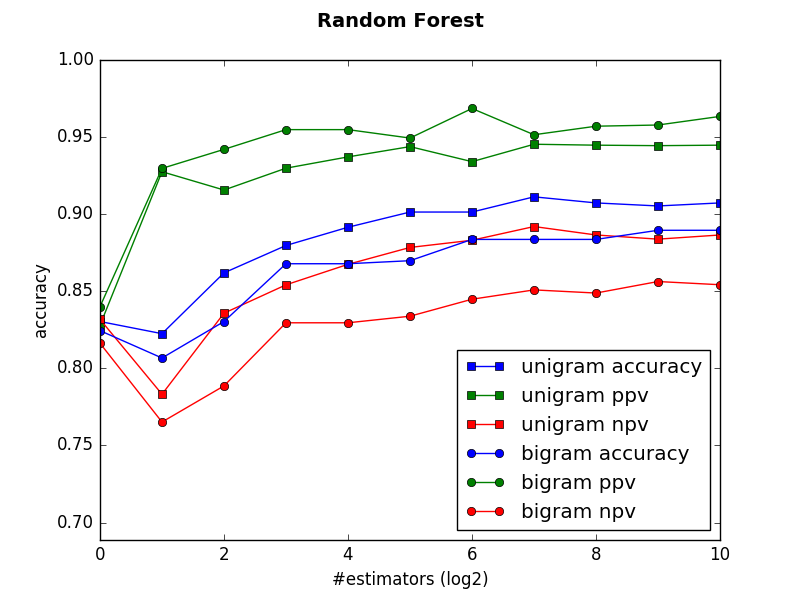
\includegraphics[trim={0 0 0 1cm},clip,width=\columnwidth]{../graphs/DisasterClassification/random_forest_unigram_vs_bigram_features.png}
	\caption{Disaster Classification - \textit{Random Forest} (Unigram vs. Bigram)}
	\label{fig:disaster_classification_rf}
\end{figure}

\begin{figure}[H]
	\centering
	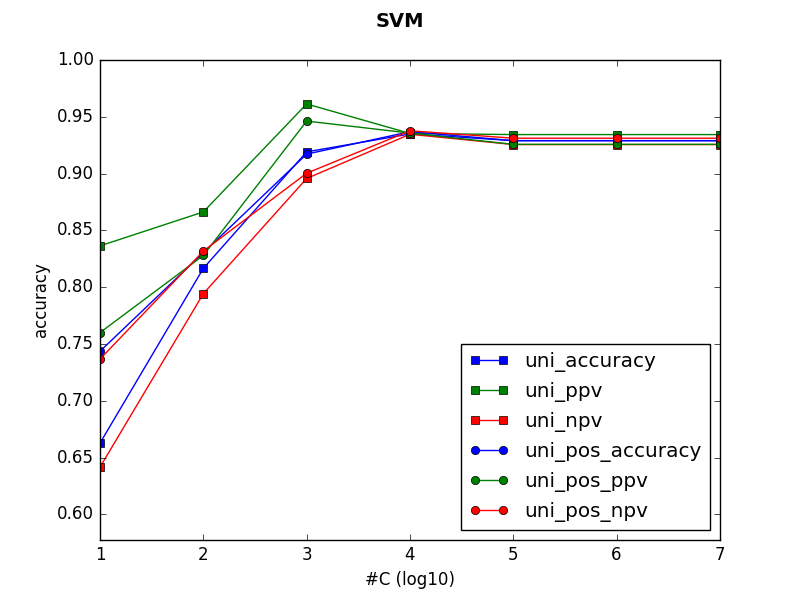
\includegraphics[trim={0 0 0 1cm},clip,width=\columnwidth]{../graphs/DisasterClassification/svm_uni_features.png}
	\caption{Disaster Classification - \textit{SVM} (Unigram vs. Unigram and POS)}
	\label{fig:disaster_classification_svm_uni}
\end{figure}

\begin{figure}[H]
	\centering
	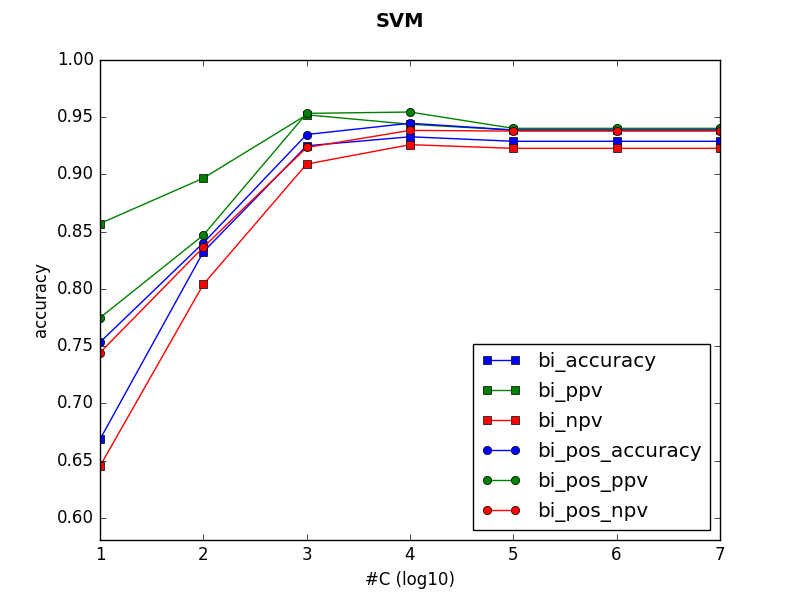
\includegraphics[trim={0 0 0 1cm},clip,width=\columnwidth]{../graphs/DisasterClassification/svm_bi_features.png}
	\caption{Disaster Classification - \textit{SVM} (Bigram vs. Bigram and POS)}
	\label{fig:disaster_classification_svm_bi}
\end{figure}

%%%%%%%%%%%%%%%%%%%%%%%%%%%%%%%%%%%%%%%%%%
\section{Sentiment Analysis of Tweets}  \label{mission2}

Sentiment analysis tasks aim to determine the writer's attitude, opinion or emotion, and are usually designed as a multi-class classification task (for example, among the labels \textit{"sad"}, \textit{"happy"}, \textit{"angry"}, etc.). Another target may be classifying the \textit{polarity} of a given text (for example, \textit{"positive"} or \textit{"negative"}).

We focused on the task of classifying disaster-related tweets to \textit{"objective"} and \textit{"subjective"} tweets. In large, we say that \textbf{\textit{"objective"}} tweets contain mere facts, undeniable truths that are universally agreed upon, and that \textbf{\textit{"subjective"}} tweets contain an opinion, sentiment or emotion towards some happening (e.g. sadness, worry, fear, sarcasm, etc.). For example, the following is an \textit{"objective"} tweet:

\begin{center}
	\parbox{190pt}{\tweet{FedEx no longer to transport bioterror germs in wake of anthrax lab mishaps http://t.co/P96rgBbaYL \#news \#phone \#apple \#mobile}}
\end{center}

and the two following tweets are \textit{"subjective"}:

\begin{center}
	\parbox{190pt}{\tweet{@denisleary Not sure how these folks rush into burning buildings but I'm grateful they do. \#TrueHeroes}}
\end{center}

\begin{center}
	\parbox{190pt}{\tweet{@canagal Good to hear it's back.. that storm's been given you guys trouble though :(}}
\end{center}

The ability to differentiate between \textit{objective} and \textit{subjective} tweets may help in identifying individuals who witnessed some disastrous event or who are in need of help.

\subsection{The Dataset}

Our dataset of 10,877 tweets did not contain a label of \textit{objective / subjective}, and we did not find any other satisfactory pre-labeled dataset of disaster-related tweets. Hence, we went on a mission to manually label all 2,100 disaster-related tweets from the dataset (that were labeled '\textit{disaster-related}' with confidence $ \ge 0.9 $).

Each tweet was independently labeled by two participants; upon disagreement the third participant broke the tie. Around 80\% of the tweets were labeled \textit{objective} while only 20\% were labeled \textit{subjective}. This results from the large amount of tweets by news agencies in the dataset.

It is worth to mention that in some cases, subtleties in writing made it hard to decide whether a tweet is \textit{"objective"} or \textit{"subjective"}. For example, the following tweet is clearly \textit{"objective"},

\begin{center}
	\parbox{190pt}{\tweet{Thunder lightening torrential rain and a power cut.}}
\end{center}

while this tweet is debatable,

\begin{center}
	\parbox{190pt}{\tweet{Thunder lightening torrential rain and a power cut!}}
\end{center}

and the following is clearly \textit{"subjective"},

\begin{center}
	\parbox{190pt}{\tweet{Thunder lightening torrential rain and a power cut! :(}}
\end{center}

\subsection{Feature Extraction}

We confirmed our hypothesis that the task of differentiating between \textit{"objective"} and \textit{"subjetive"} disaster-related tweets can be achieved without examining the vocabulary of tweets, but merely by using POS tags and the following metadata features, which we extracted for each tweet:


\begin{itemize}[noitemsep, nolistsep]
	\item Presence and number of exclamation marks.
	\item Presence and number of question marks.
	\item Presence of URLs.
	\item Presence of emoticons (extracted using \texttt{emoticon.py}, Twitter NLP framework \cite{twitter_nlp}).
	\item Number of digits.
	\item Number of capitalized words.
	\item Number of capital letters.
	\item Number of punctuation marks and symbols (!"\#\$\%\&'()*+,-./:;<=>?@[\textbackslash]\^\_`\{\}\textasciitilde).
	\item Tweet's length.
	\item POS tag statistics:
		\begin{itemize}[noitemsep, nolistsep]
			\item Number of adjectives.
			\item Number of verbs.
			\item Number of adverbs.
			\item Number of pronouns.
			\item Number of proper nouns.
			\item Number of possessive endings.
		\end{itemize}
\end{itemize}

\subsection{Results}
We trained \textit{SVM} and \textit{Random Forest} classifiers for this task, using $ C=10^4 $ as a penalty constant for \textit{SVM} and 128 estimators for \textit{Random Forest}.

Once again the dataset was divided into train (90\%) and test (10\%) sets. Each classification method was tested with the previously mentioned features, using feature selection with \textit{ANOVA F-test} model. We repeated the test several times, each time increasing the number of $K$ best features selected by the feature selection model (out of 18 features total), and measuring accuracies (as mentioned in the previous \textit{Identification} task). Our goal was to find which features are the most expressive for the task. We used the measures of total accuracy, \textit{PPV} and \textit{NPV}.

\paragraph{Random Forest.} Looking at the \textit{Random Forest} results (fig.  \ref{fig:obj_sub_classification_rf}), we can see that best total accuracy is achieved with 13 features, so for \textit{NPV}, but best \textit{PPV} is achieved with only 1 feature (might be due to the biased dataset). The most expressive features used are:
number of exclamation marks, presence of exclamation mark, presence of question mark, presence of URL, presence of emoticon, number of digits, number of capital letters, number of punctuation marks and symbols, tweet's length.

\paragraph{SVM.} Looking at the \textit{Random Forest} results (fig.  \ref{fig:obj_sub_classification_svm}), we can see that best total accuracy is achieved with 4 features only, so for \textit{NPV}, but best \textit{PPV} is achieved with only 1 feature as well (again, might be due to the biased dataset). The most expressive features used are:
number of exclamation marks, presence of URL, presence of emoticon, number of punctuation marks and symbols.

Table \ref{tab:obj_sub_classifiaction_best_results} presents the best measurement result for each classifier. Best total accuracy result (87.1\%) is achieved with \textit{Random Forest} classifier using 13 features. \\

\begin{table}[H]

	\begin{center}
		\scalebox{0.8}{
			\begin{tabular}{c | c | c | c | c }
				& \textbf{RF (1)} & \textbf{RF (13)} & \textbf{SVM (1)} & \textbf{SVM (4)} \\ \hline
				accuracy & 0.805 & 0.871 & 0.805 & 0.848 \\
				ppv & 0.905 & 0.890 & 0.905 & 0.874 \\
				npv & 0.500 & 0.750 & 0.500 & 0.667 \\
			\end{tabular}
		}
	\end{center}
	\caption{Objective/Subjective Classification Best Results (in parentheses - number of features used)} 	\label{tab:obj_sub_classifiaction_best_results}
\end{table}

\begin{figure}[H]
	\centering
	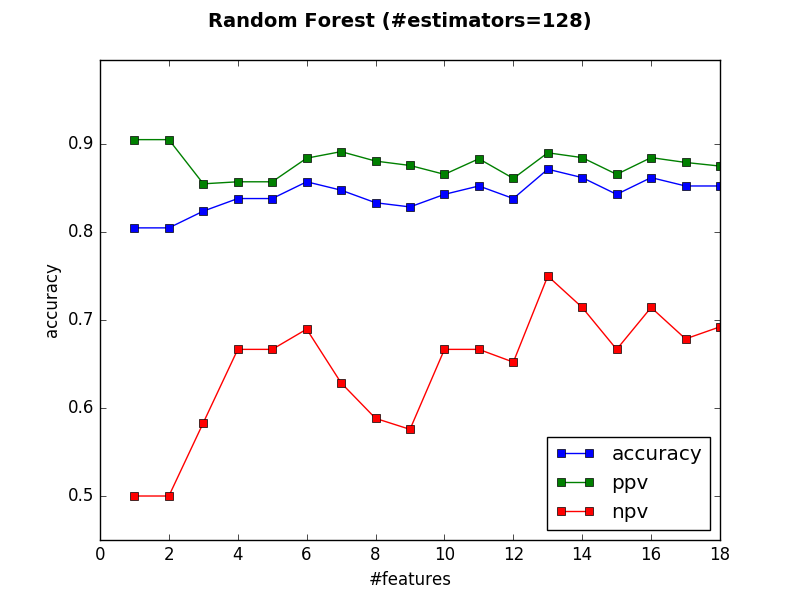
\includegraphics[width=\columnwidth]{../graphs/SentimentAnalysis/random_forest.png}
	\caption{Objective/Subjective Classification - \textit{Random Forest}}
	\label{fig:obj_sub_classification_rf}
\end{figure}

\begin{figure}[H]
	\centering
	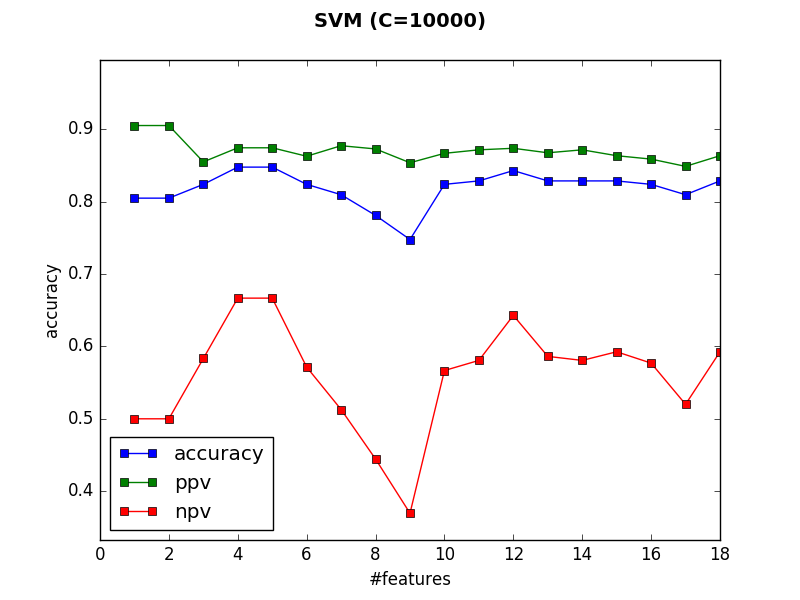
\includegraphics[width=\columnwidth]{../graphs/SentimentAnalysis/SVM.png}
	\caption{Objective/Subjective - \textit{SVM}}
	\label{fig:obj_sub_classification_svm}
\end{figure}

%%%%%%%%%%%%%%%%%%%%%%%%%%%%%%%%%%%%%%%%%%
\section{Named-Entity Recognition in Tweets}  \label{mission3}


We aim to extract relevant information from tweets we previously classified as disaster-related. Named-entity recognition (NER) allows us to extract names of people, organizations, locations and time expressions. Ritter et al., (\textit{Named Entity Recognition in Tweets: An Experimental Study}, 2011 \cite{Ritter11}) provide a method to extract named entities out of \textit{tweet corpora}, by using a Twitter-specific POS tagset (similar to the tagset we used in our previous classifiers). In this section, we present our attempt to use the Groningen Meaning Bank (GMB), which was trained on news and articles (rather than Twitter corpora), and extract named entities out of tweets.

\paragraph{Groningen Meaning Bank (GMB).}
In order to develop a named-entity recognizer we used the Groningen Meaning Bank\endnote{\textbf{"Groningen Meaning Bank" Dataset by University of Groningen}: comprises of thousands of texts in raw and tokenized formats, tags for part of speech, named entities and lexical categories, and discourse representation structures compatible with first-order logic. \url{http://gmb.let.rug.nl/}} - a large corpus containing thousands of texts in raw and tokenized formats, POS tags, named entities by lexical categories and much more. The top level categories of the corpus are:

\begin{itemize}[noitemsep, nolistsep]
	\item \textbf{geo} - Geographical Entity
	\item \textbf{org} - Organization
	\item \textbf{per} - Person
	\item \textbf{gpe} - Geopolitical Entity
	\item \textbf{tim} - Time indicator
	\item \textbf{art} - Artifact
	\item \textbf{eve} - Event
	\item \textbf{nat} - Natural Phenomenon
\end{itemize}

We used only the top-level categories, which are sufficient for extracting relevant information on disasters. As the database contains POS tags in NLTK format, we used NLTK to create POS tags for our tweets, rather than the Twitter tagger by Gimpel et al. \cite{POS-Tagging}.

\paragraph{Capitalization.} A key feature for recognizing named entities capitalization. In case of tweets, which are written by non-professional writers, capitalization is much less reliable, and differs in style between twitter users. Capitalization irregularities in tweets can be the result of spelling errors, or may be used to express the writers sentiment or emotion.

To overcome this obstacle, we implemented an approach similar to that of Ritter et al., 2011 \cite{Ritter11}, and converted our data to all lower-case. Using capitalized words as features caused a great shift in the results - entities of different types where often grouped together, and non-entities where often identified as such. Manipulations on the capitalization feature extractor - such as announcing a word as capitalized, only if its surroundings are not all capitalized, performed poorly as well. By neutralizing this feature, and converting all the tweets to lower case letters, the classifier performance increased significantly.

\subsection{Results}

Four main categories of the GMB corpus are relevant for our purposes - \textit{location} (\textbf{geo}), \textit{organization} (\textbf{org}), \textit{persons} (\textbf{per}) and \textit{geopolitical entity} (\textbf{gpe}). A fifth category, \textit{time} (\textbf{tim}), was somewhat ambiguous - as it described both time entities and irrelevant ones. Other categories did not manage to reach any level of internal agreement on any entity.

By using the GMB corpus as the training data, we performed named entity recognition on the previously used dataset of 10,877 labeled tweets. From those tweets, we singled out only those who were labeled as disaster-related. The main results were:

\begin{itemize}[noitemsep, nolistsep]
	\item \textit{Geographical Entity} - California and Hiroshima were the dominant entities, as there were tweets about disasters in those places, followed by Japan, India, south, and Saudi Arabia.
	\item \textit{Organization} - This category was composed of news companies, such as ABC and BBC, and by examples such as Washington, which was treated as an organization representing the U.S (rather than the city/state). Many user references are marked as an organizations as well.
	\item \textit{People} - The only pure result in this category is Obama.
	\item \textit{Geopolitical Entity} - Composed mostly of user references, and nationalities - Israeli, Turkish and more.
	\item \textit{Time Indicator} - ranged from a description of current events - wildfire or typhoon, to description of the 70th anniversary of Hiroshima atom bombing. Included some specific time references, such as Wednesday.
\end{itemize}

From those results, we can learn the location, nationality of involvement, associated organizations, and type of the disaster. We classified and manually checked the results in order to learn the false-alarm rate of our implementation, as presented in table 
 \ref{tab:named_entity_recognition_success_rate}. The most common entities are California, Hiroshima, ABC, Turkey, Northern, severe, refugio, Japan, Obama and ABC-News.

\begin{table}[H]
	\begin{center}
		\scalebox{0.8}{
			\begin{tabular}{c | c | c | c | c | c}
				  & $ \textbf{geo} $ & $
				  \textbf{org} $ & $ \textbf{per} $ & $ \textbf{gpe} $ & $ \textbf{tim} $ \\ \hline
				Total & 337 & 306 & 41 & 865 & 787  \\
				Success Rate & 80\% & 57\% & 76\% & 49\% & 27\% \\
			\end{tabular}
		}
	\end{center}
	\caption{Named Entity Recognition Success Rate}
	\label{tab:named_entity_recognition_success_rate}
\end{table}


%%%%%%%%%%%%%%%%%%%%%%%%%%%%%%%%%%%%%%%%%%
\section{Experimenting with Recent Tweets} \label{recent-tweets-results}

In the last part of our work we tested our classifier that identifies \textit{disaster-related} tweets and the NER classifier on real data that was recently posted on Twitter. We used Twitter's Search API that allows developers to browse tweets that were posted during the previous 7 days, and filter them according to various categories such as language, location (by coordinates), keywords and more.

\paragraph{The Data.} We created the following three tweet dataset:

\begin{itemize}[noitemsep, nolistsep]
	\item\textbf{Houston} - 1,501 tweets posted in the \textit{Houston, TX} area during 29 Aug. - 3 Sept., containing at least one of the words [\tweet{water, drown}] and 500 random tweets
	\item\textbf{Miami} - 1,001 tweets posted in the \textit{Miami, FL} area during 9 Sept., containing at least one of the words [\tweet{evacuate, stay, safe, car}] and additional 150 random tweets
\end{itemize}

For both datasets we avoided "re-tweeted" tweets (\tweet{RT}), to prevent repetitions of popular tweets.\\

For each of the datasets we used our classifier (see section \ref{mission1}) to take only \textit{disaster-related} tweets. We checked the performance of our NER classifier by running it on the disaster-related tweets in each dataset, and presenting the most popular named-entities found. We ran both our NER classifier (trained on the GMB dataset), and the Twitter-oriented NER by Ritter et al. \cite{Ritter11}.

The most popular entities among the \textbf{Houston} tweets:

\begin{itemize}[noitemsep]
	\item\textbf{Our NER} - \tweet{Houston, Mandatory, Twitter, Harvey, Water, Beaumont, Air Alliance, Info, Houston Water, Hurricane Harvey}
	\item\textbf{Ritter et al.} - \tweet{Houston, Twitter, Harvey, Hurricane Harvey, Google Maps, Beaumont, Houston Water, Katy, Air Alliance Houston, Texas}
\end{itemize}

The most popular entities among the \textbf{Miami} tweets:

\begin{itemize}[noitemsep]
	\item\textbf{Our NER} - \tweet{Florida, Irma, Miami, Twitter, Hurricane, Hurricane Irma, Leaving, Floridians arent, Cuba and Hurricaneirma}
	\item\textbf{Ritter et al.} - \tweet{Florida, Irma, Miami, Twitter, Hurricane Irma, Cuba, Florida Keys, tampa, Key West, Paramount Pictures Settles}
	
\end{itemize}


The results show that both NER methods manage to identify the two recent large scale hurricanes that affected Houston (Hurricane Irma) and Miami (Hurricane Harvey).
The comparison starts to fail when comparing the uncommon named entities; this is not surprising, since we expected Ritter's method, which is adjusted to Twitter corpora, to be superior. However, our method is sufficient for understanding the trivial details of large-scale disasters - location and type of disaster.

%%%%%%%%%%%%%%%%%%%%%%%%%%%%%%%%%%%%%%%%%%
\section{Conclusions}

We have developer a classifier that identifies \textit{disaster-related} tweets among other tweets. We addressed the uniqueness of tweet corpora, and integrated in our work Twitter-oriented NLP tools for tokenization, part-of-speech tagging and named-entity recognition. Our classifier achieved around 94\% accuracy. We have also developer another classifier trained to distinguish between \textit{"objective"} and \textit{"subjective"} tweets. \todo{explain why SVM worked better in the first classifier, while RF worked better in the second one}.

In the last part of our work we demonstrated our classifier on recent tweets, from which we extracted named entities and found some locations and names related to recent hurricanes.

As for future work, we believe that this experiment with disaster-related tweets can be improved and expanded to create a system that detects emergencies in real-time by analyzing the live stream of tweets, using Twitter's Stream API; further improvements in the NER phase may help in analyzing the temporal and spatial pattern of an event; improvements in the sentiment analysis phase may help in identifying individuals who are in need of help.

The code of our project is available at \url{https://github.com/glrn/nlp-disaster-analysis}.


%%%%%%%%%%%%%%%%%%%%%%%%%%%%%%%%%%%%%%%%%%

{\footnotesize \bibliographystyle{acm}
\bibliography{references}}

\theendnotes

\end{document}







